\documentclass[letterpaper, 11pt, twocolumn]{article}
\usepackage{graphicx}
\usepackage{amsmath}
\usepackage{float}
\usepackage{geometry}
\geometry{letterpaper, margin=20mm, nohead}
\linespread{0.9}


\graphicspath{{./pics/}}
\begin{document}

\title{\vspace{-10mm} 6.013 Final Project Report}
\author{Andres Erbsen, Justin Graves, Dimitris Koutentakis}
\date{\today}
\maketitle
\vspace{5mm}
% \tableofcontents
% \clearpage
\section{Abstract}
From 6.013 we learned that transmission lines can resonate at certain
frequencies and create standing waves based on the geometry and reflection
coefficients at the boundaries of the lines. We used this concept to design,
build, and characterize two band-pass filters (achieving 30dB stop-band
attenuation) based on TEM resonators and two band-stop filters that produce a
smith chart short at the stop frequency (achieving 45dB attenuation).

\section {Introduction}
Designing filters using discrete components has its limitations. Basic filters are built using discrete components such as capacitors and inductors in which their constitutive voltage-current laws are only time dependent. In 6.013, we learned that if the dimensions of your circuit are comparable to the wavelength of your of your signal, that phase changes in voltages and currents become significant. As frequency of a signal increases, the wavelength decreases and for anything in the radio frequency $f > 300 MHz$ our wavelength will be less than a meter. These introduced phase changes from having dimensions comparable to the wavelength, will produce maximas and minimas in voltages and currents along the path your signals travels. The model for discrete reactive components only depend on time but with the introduction of phase changes we now need reactive components that both depend on time and space, which are called distributed elements. It must also be said that with discrete reactive components, capacitors and inductors, the range of possible reactive values is limited but in not the case with distributed components. 


\section{Approach}
In order to design our filters, we had to apply some of the basic knowledge we acquired in the lectures towards the end of the semester. More specifically, we had to apply knowledge regarding transmission line resonators as well as smith charts and stubs.
\\
By calculating the dimensions for our given substrate and target frequencies we were able to build the filters desired. The filters that we ended up building are:
\begin{itemize}
    \item A short-short half wave resonator built with the dimensions of the original substrate board,
    \item A short-short half wave resonator for $f=2.4 GHz$,
    \item A single stub band-stop resonator, and
    \item A multiple stub band pass approximation filter
\end{itemize}
\subsection{Half wave resonator band-pass filter}
For the first short-short half-wave resonator, we used the dimensions of the original board given. More specifically, we used the width of the board, $D=7.7cm$ and $\delta$ very small (\(\delta<0.8cm\) in order to maximize our $Q$. Given the width of our board and the material with $\epsilon_r=2.33$, we calculated a wavelength of \(\lambda_0=2\cdot D \cdot\sqrt(\epsilon_r)=23.5cm\), corresponding to a resonant frequency of $f=\frac{c}{\lambda_0}=1.277GHz$.
% \begin{align*}
%     D=7.7cm &\Rightarrow \frac{\lambda_n}{D}=7.7cm \\
%     \lambda_0=7.7cm\cdot2\cdot\sqrt{2.33}&\Rightarrow \lambda_0=23.5cm \\
%     f=\frac{3\cdot10^{8}}{23.5\cdot10^{-2}} &\Rightarrow f=1.277 GHz
% \end{align*}

% \begin{figure}[H]
%     \centering
%     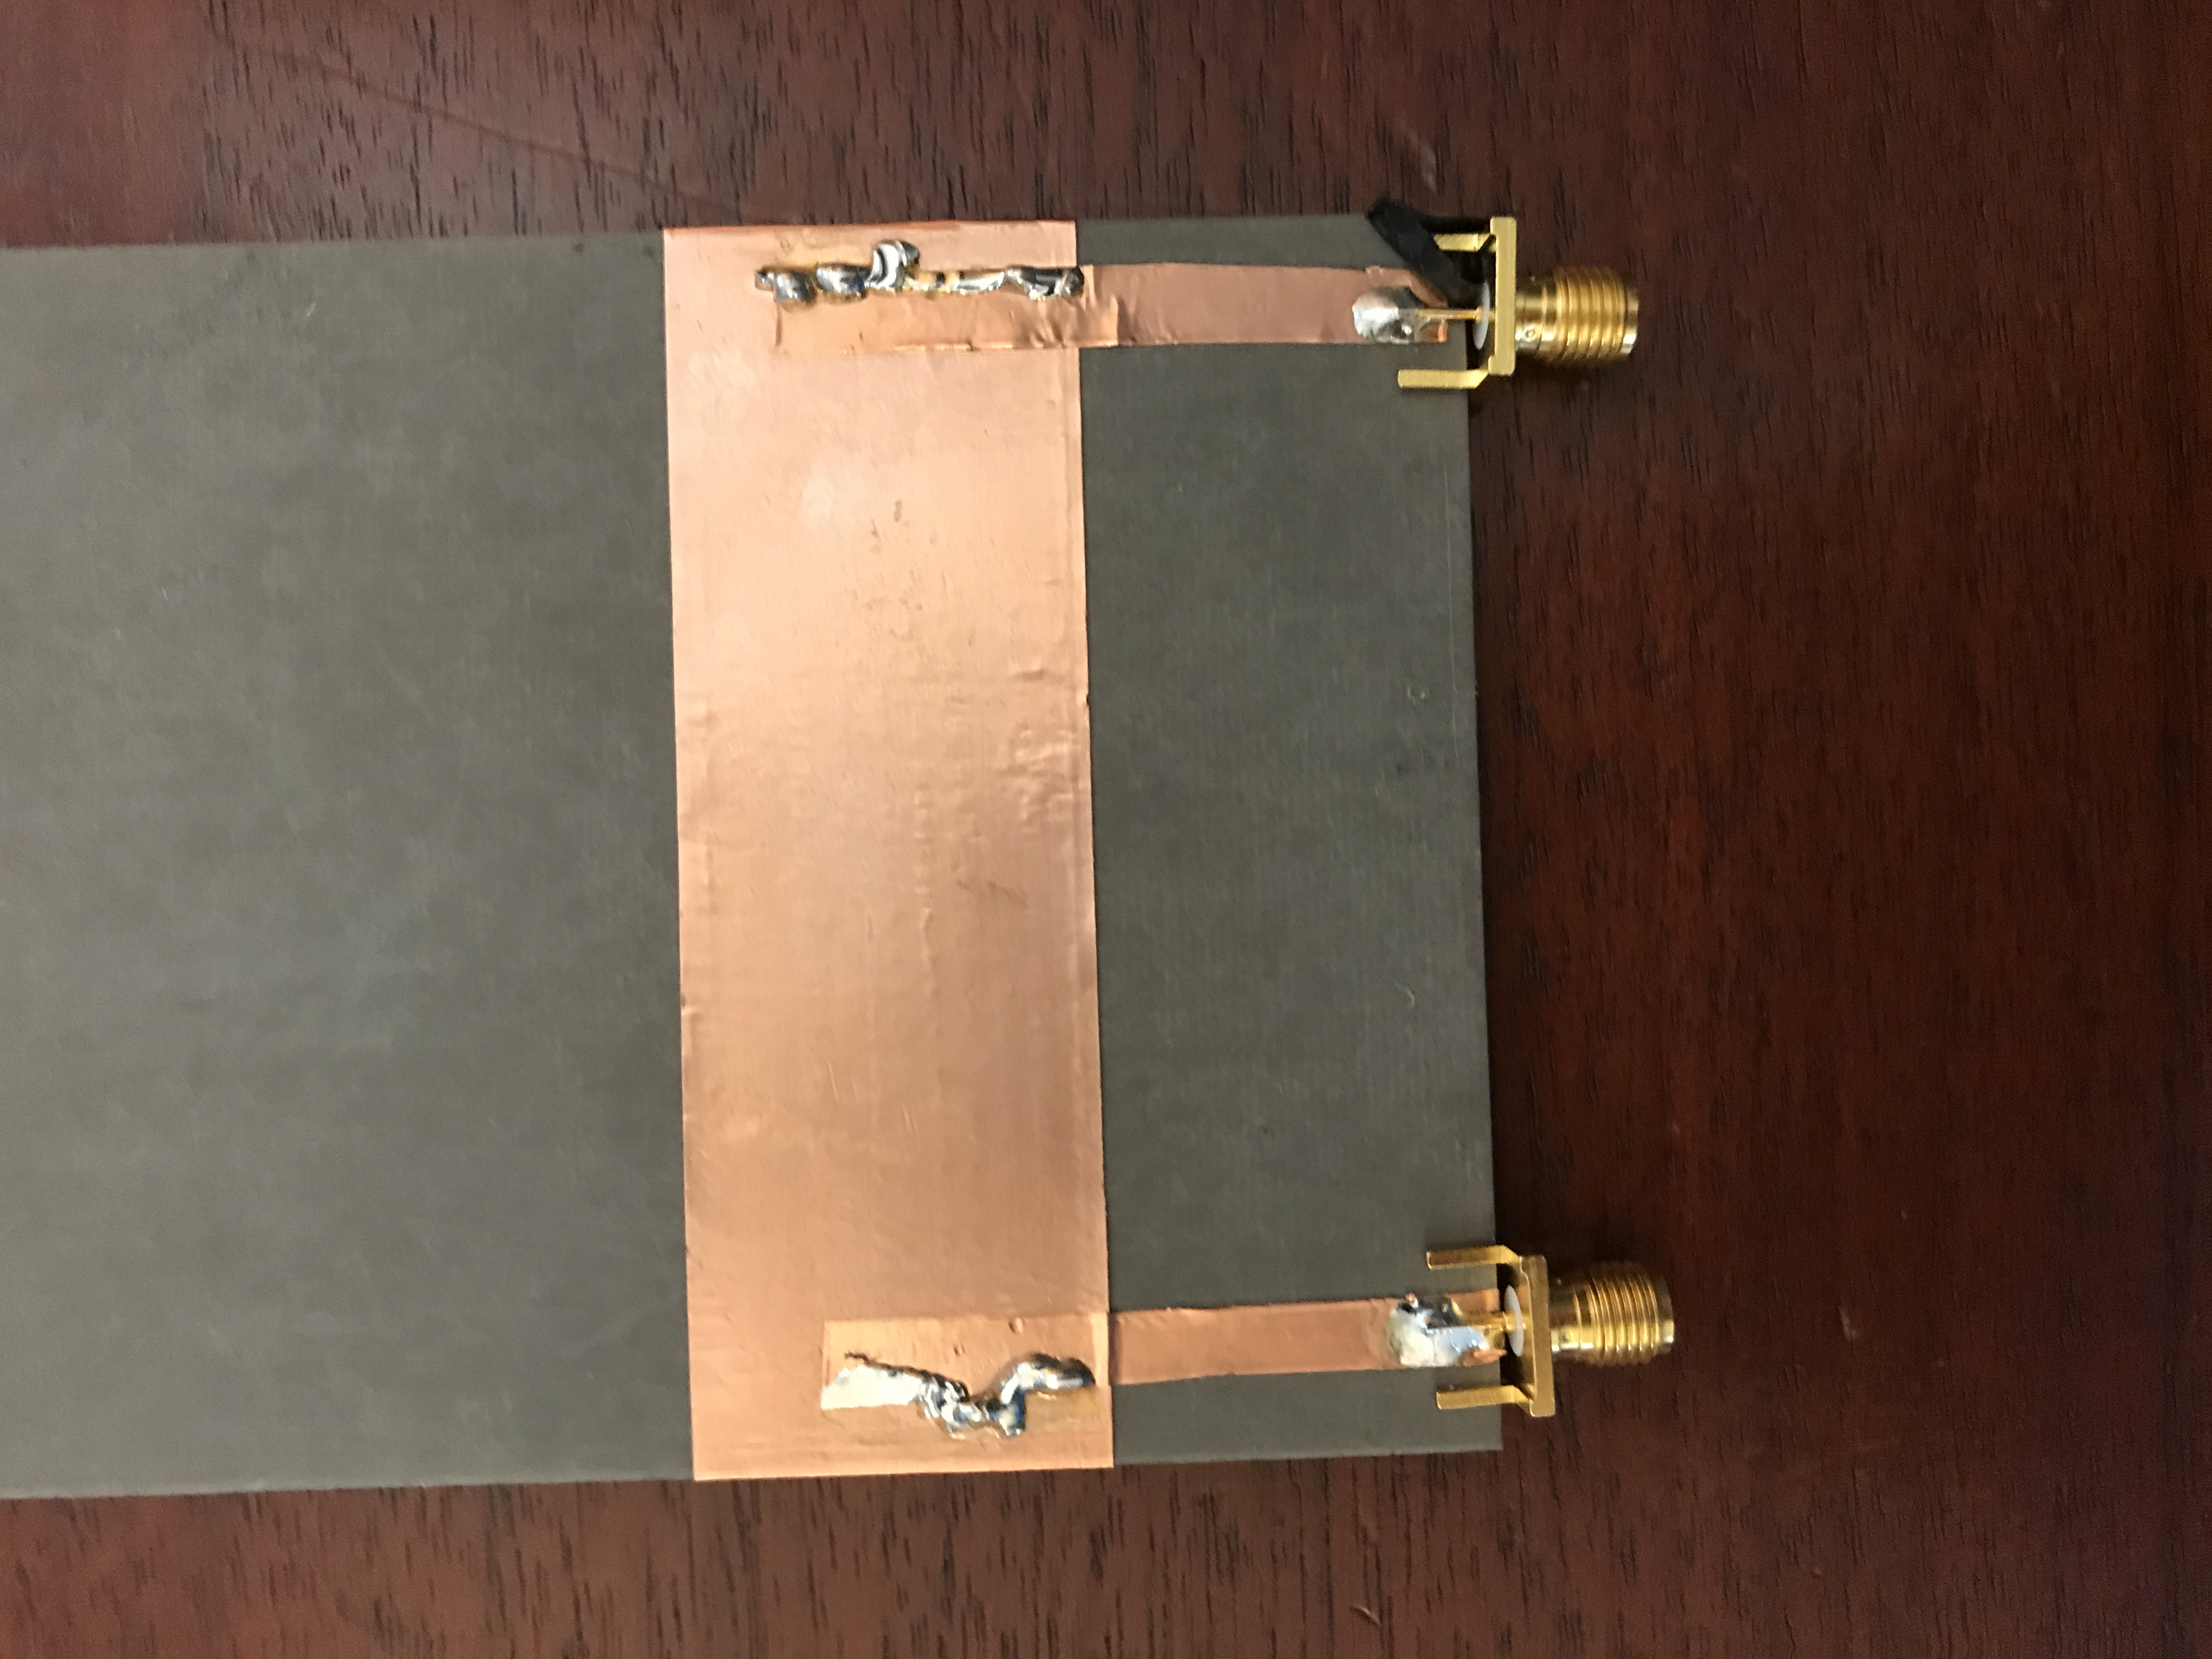
\includegraphics[width=0.8\textwidth, angle = 270]{filter1}
%     \caption{Original width half-wave resonator filter}
% \end{figure}
% \clearpage
\subsection{2.4 GHz half-wave resonator band-pass filter}
In order to build a filter that would work in Wi-Fi range (or at our radar's working frequency), we had to design and build a filter that would only let signal through at around 2.4 GHz. In order to do so, we repeated the above procedure after first calculating the desired length by using: \(D=\frac{m\cdot\lambda_n}{2}\),\(\lambda_n=\frac{\lambda_0}{n}\), \(m=1\),\(\epsilon_r=2.33\), and \(\mu_r=1\). This calulation resulted in a desired length of \(D=0.0409m\). Then we cut the substrate and copper tape appropiately and soldered the connectors. 

% After cutting the substrate boards at the calculated dimensions, we had the following filter:
% \begin{figure}[H]
%     \centering
%     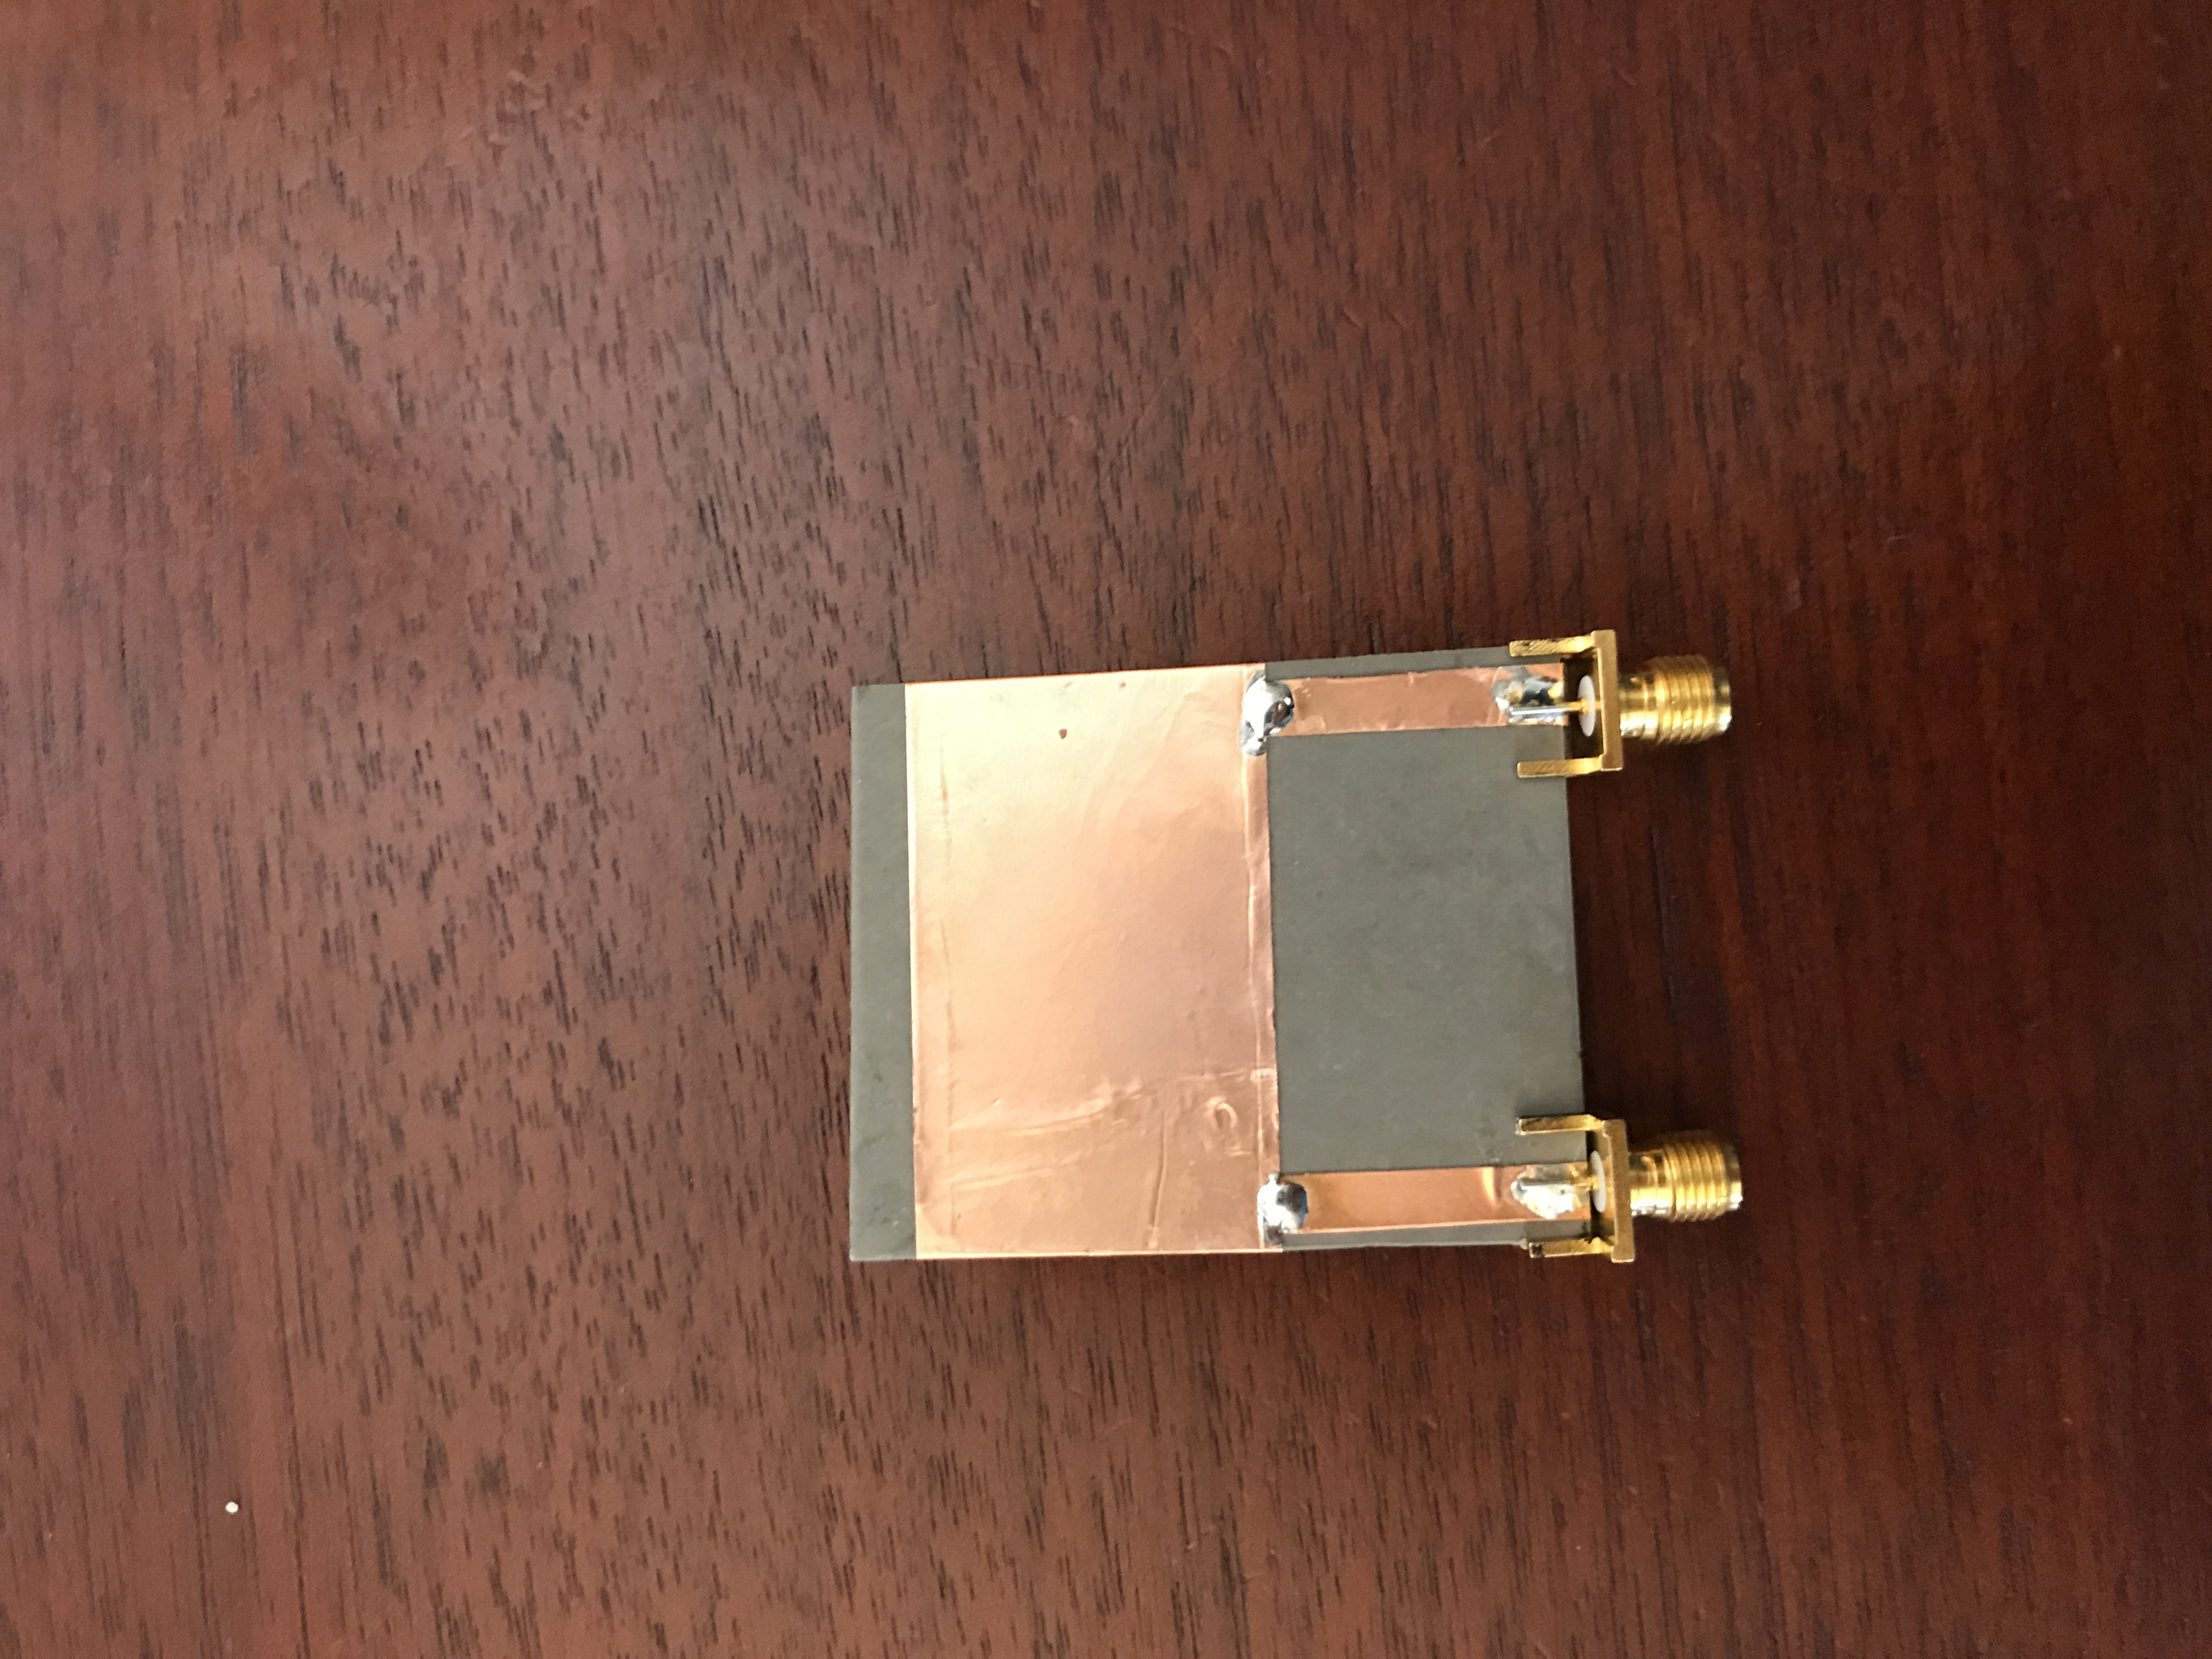
\includegraphics[width=0.8\textwidth, angle = 270]{filter2}
%     \caption{2.4GHz half-wave resonator filter}
% \end{figure}

\subsection{Single stub band-stop filter}
In order to make a band-stop filter, we decided to make a single \(\frac{\lambda}{4}\) stub on a \(50 \Omega\) line. That is designed to transform the open at the end of the stub to a short in parallel with the line which would result in no signal at that frequency. In order to find the correct length, we calculated the wavelength on the substrate, which is \(\lambda=\frac{c/\sqrt{2.33}}{2.4GHz}=0.082m=8.2cm\). That means that our stub has to be \(l=\frac{\lambda}{4}=\frac{8.2}{4}=2.025cm\).
\subsection{Multiple stub band-pass filter}
One other design we developped was a multiple frequency band-stop filter. In order to achieve an approximation of a wide band-pass filter with very sharp edges, we designed a filter that would have multiple band-stop frequencies. 
\section{Results}

\subsection{Half wave resonator Band-Pass filter}
As seen in the yellow line, the short-short band pass filter described first above, returned a relatively promising behavior which is part of the reason we decided to proceed with the same design for the Wi-Fi range. More specifically, the first resonant frequency gave us an attenuation of only around 15 dB at 1.45 GHz. The other resonant frequencies performed even better with attenuations at 8 and 3.5 dB at frequencies of approximately 2.8 and 4.15 GHz respectively.
% \begin{figure}
%     \centering
%     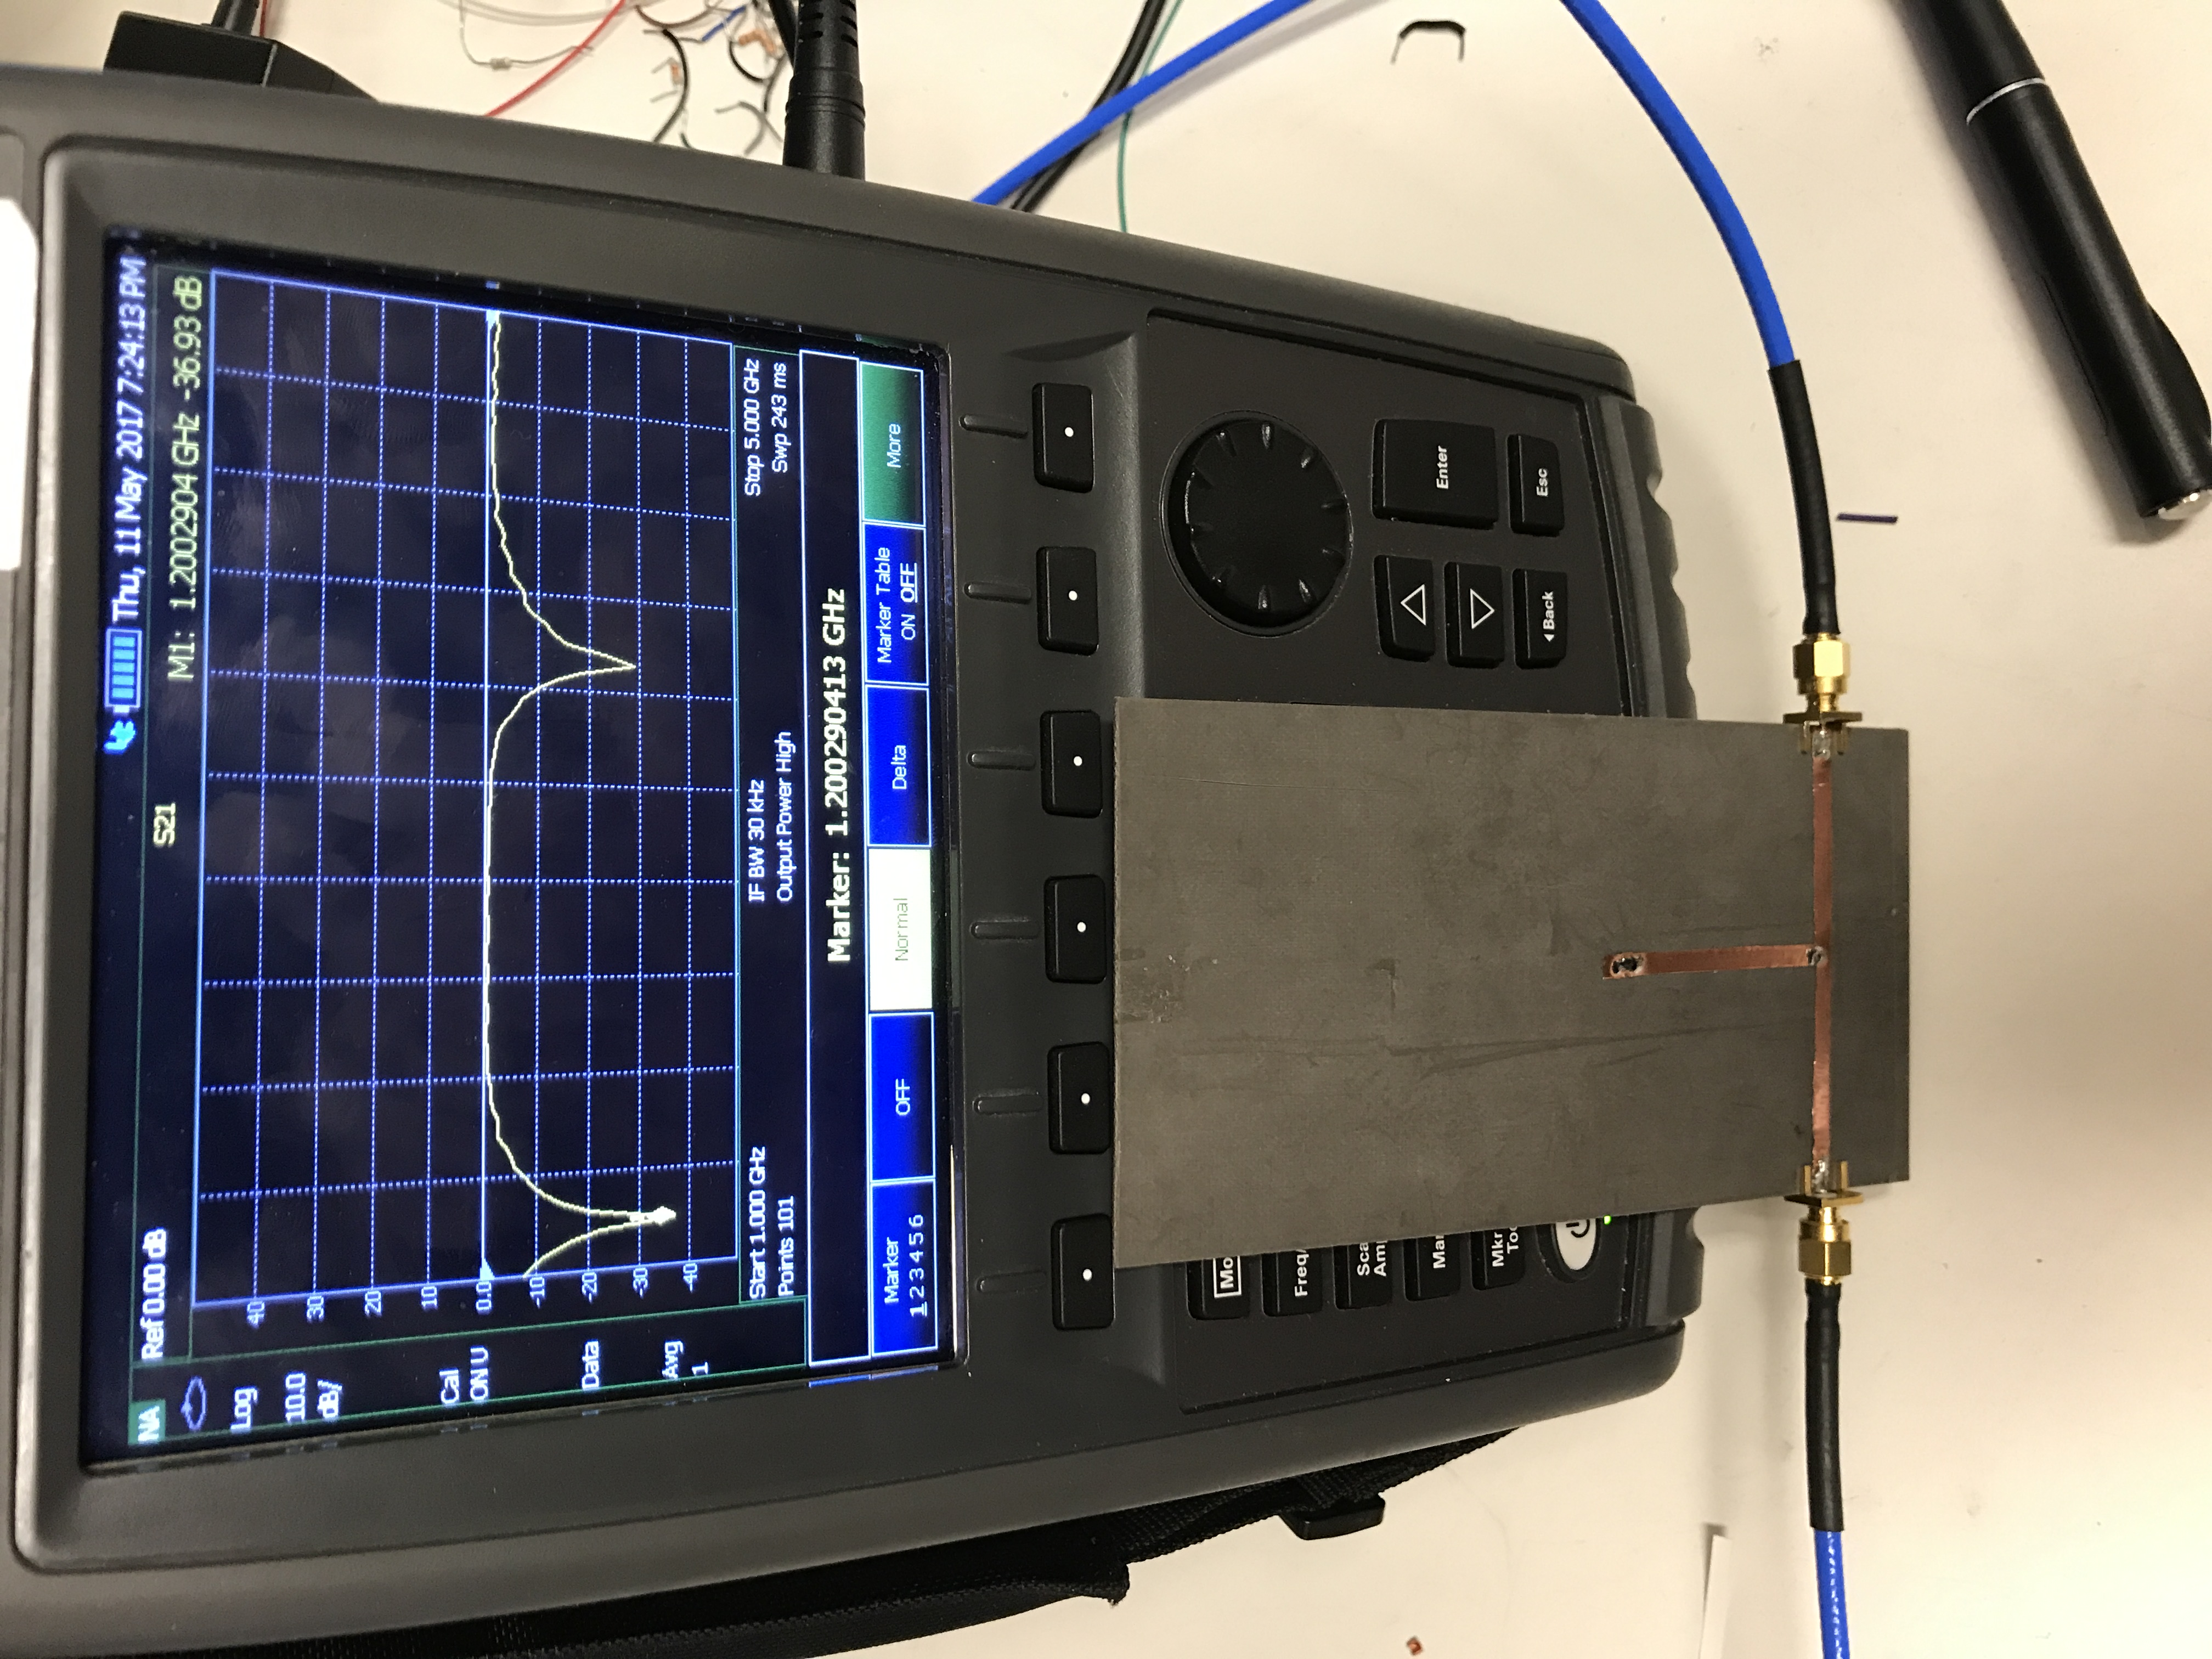
\includegraphics[width=0.8\textwidth, angle=270]{1stub}
%     \caption {single stub measurements}
% \end{figure}
% \subsection{Short-short 2.4 GHz resonator}

\subsection{2.45 GHz half-wave band-pass filter}
The 2.45 GHz worked out much better in the experiments we conducted because of the more careful dimensioning and manufacturing of the filter. As it can be seen in the figure attached, the red line representing this filter is attenuated only by 2.6 dB at 2.45 GHz, while the rest (with the exception of the second resonant frequency which is attenuated by 1.4 dB at 4.95 GHz), generally provides more than 30dB attenuation. This performance was exceptionally promising for the filter desing.  


\subsection{Single stub band-stop filter}
The single-stub quarter wavelenth 2.4 GHz band-stop filter produced again a surprisingly good output. As demonstrated by the blue line on the plot, this filter returned a very sharp "dip" at 2.375 GHz, attenuating the signal by 36dB. The attenuation far from the cut-off frequency was virtually zero. The only problem we faced with this design is in trying to attenuate Wi-Fi signal, as the stub would act as an antenna since we could not properly shield it. This was partially solved by shielding it in aluminum foil (purple line). 

\subsection{multiple stub band-pass filter}
The multiple band-stop frequency quarter-wavelength stub filter is represented by the green line on the graph. This filter resulted in a wide enough band with very sharp edges and virtually zero attenuation at around 2.4-2.5 GHz which was the respone we were looking for. In addition to that, one can see low-attenuation peaks at frequencies not attenuated by the stubs or their resonant frequencies. 

\begin{figure}[H]
    \centering
    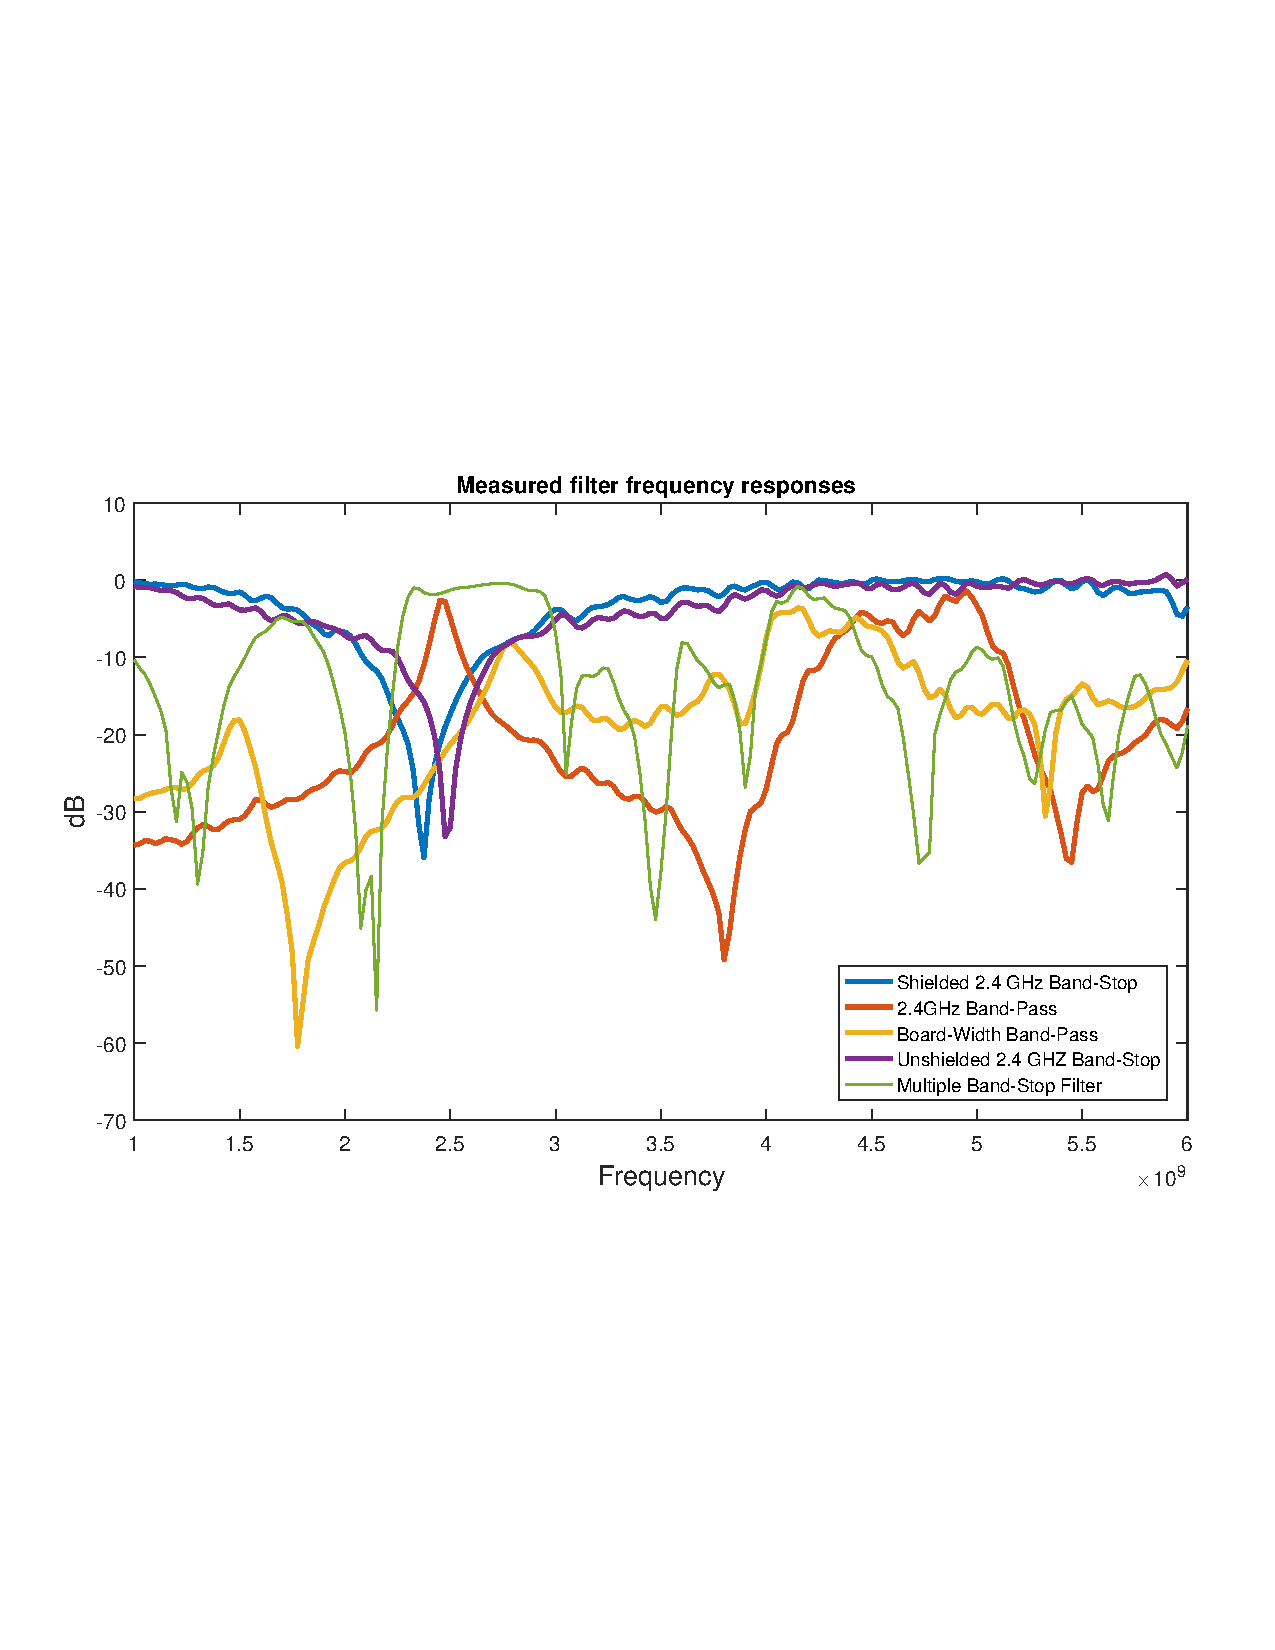
\includegraphics[trim={0.5cm, 7.8cm, 0.2cm, 8cm}, clip=true, width=0.55\textwidth]{graph.pdf}
    \caption{Matlab plot of VNA-measured filter responses}
\end{figure}
\section{Conclusion}
describe
\end{document}

